\section{ОТРИМАНІ РЕЗУЛЬТАТИ}

У програмному продукті використовуюються методи математичної лінгвістики,
тобто тієї галузі лінгвістики,
що займається вивченням структури природних мов, для виведення та встановлення
певних правил та мовних законів. Завдяки цьому ми можемо аналізувати збережені дані.

Оскільки архітектура програми є досить гнучкою, можна обирати будь-які
параметри для порівняння, для будь-якою мови корпусу текстів Universal
Dependencies.

\subsection{Корпус української мови}
Завдяки кінцевому програмному продукту було проаналізовано 7060 речень 
та, загалом, 122000 токенів, які мають синтаксовий шар.
Для аналізу використовувалися різні тексти, для того, щоб охопити максимальну
пвдмножину всієї мови: статті, новини, дописи, підручники, листування, казки,
худпроза — і сучасні, і класичні~\cite{bib12}.

Результатом аналізу корпусу української мови стали наступні законормрності,
які відображені у графіках.

На рисунку~\ref{img:uk_upos} проілюстровано графік частот універсальних
частин мови, тобто upos, де видно, що у корпусі всього 17 унікальних
частин мови, де найпопулярнішою є іменник, який зустрічається в різних
місцях майже 10000 разів.

\begin{figure}[ht]
  \begin{center}
    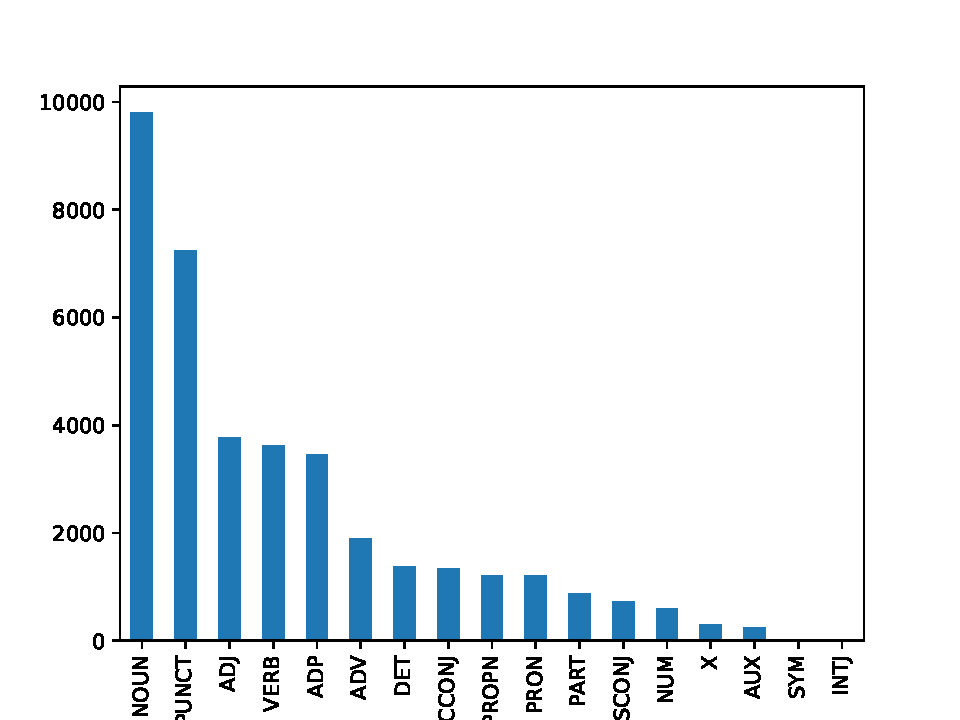
\includegraphics[width=\linewidth]{chart_uk_upos.pdf}
  \end{center}
  \caption{Графік частот універсальних частин мови}
  \label{img:uk_upos}
\end{figure}

\newpage
Порівнявши такий розподіл із законом Зіпфа, ми можемо зрозуміти, що
універсальні частини мови йому не підлягають.

На відміну від універсальних частин мови, порівнявши сигнатуру, де за основу
взяті і універсальна частина мови і її синтаксичне відношення, отримаємо
розподіл, який майже точно накладається на розподіл Зіпфа,
рисунок~\ref{img:uk_deprel_upos}. Також на цьому рисунку можемо побачити, що 
всього таких сигнатур у корпусі 37722, при чому унікальних
тільки 178.

\begin{figure}[ht]
  \begin{center}
    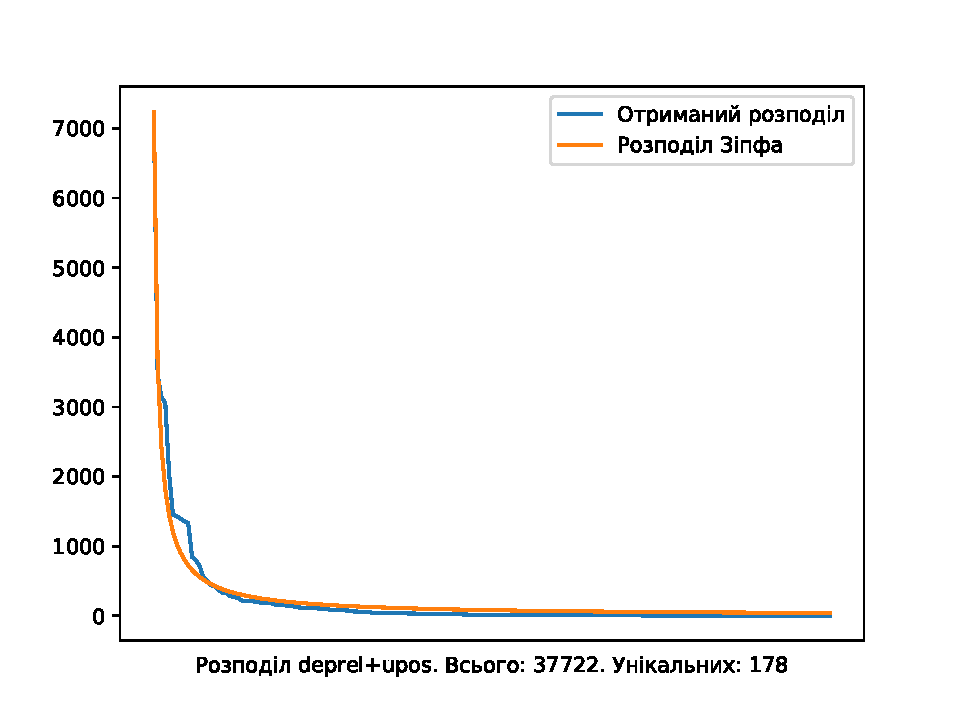
\includegraphics[width=\linewidth]{chart_uk_deprel_upos.pdf}
  \end{center}
  \caption{Розподіл частин мови та універсального відношенння}
  \label{img:uk_deprel_upos}
\end{figure}

\newpage

\begin{multicols}{2}
\begin{figure}[H]
  \begin{center}
    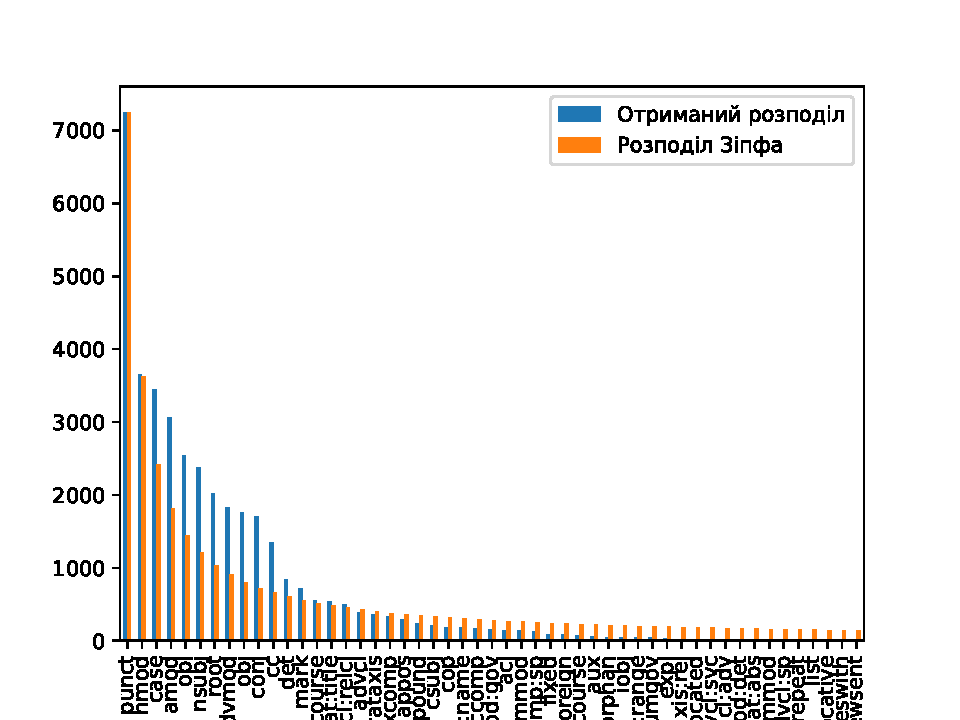
\includegraphics[width=\linewidth]{chart_uk_deprel.pdf}
  \end{center}
  \caption{Розподіл універсальних відношенннь}
  \label{img:uk0}
\end{figure}

\begin{figure}[H]
  \begin{center}
    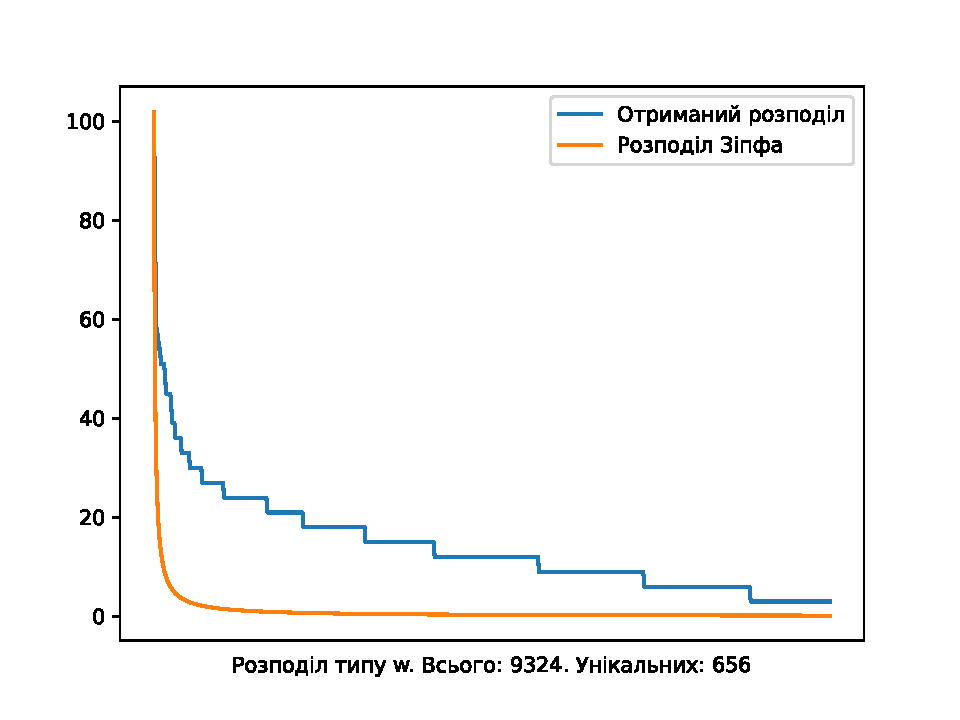
\includegraphics[width=\linewidth]{chart_uk_type_w.pdf}
  \end{center}
  \caption{Розподіл піддерев токенів, що ростуть вшир}
  \label{img:uk3}
\end{figure}

\end{multicols}

\newpage

\subsection{Корпус іспанської мови}
Проаналізувавши корпус іспаномовних текстів, який щонайменше у 8 разів
більший за корпус україномовних текстів, отримаємо:

\begin{multicols}{2}
\begin{figure}[H]
  \begin{center}
    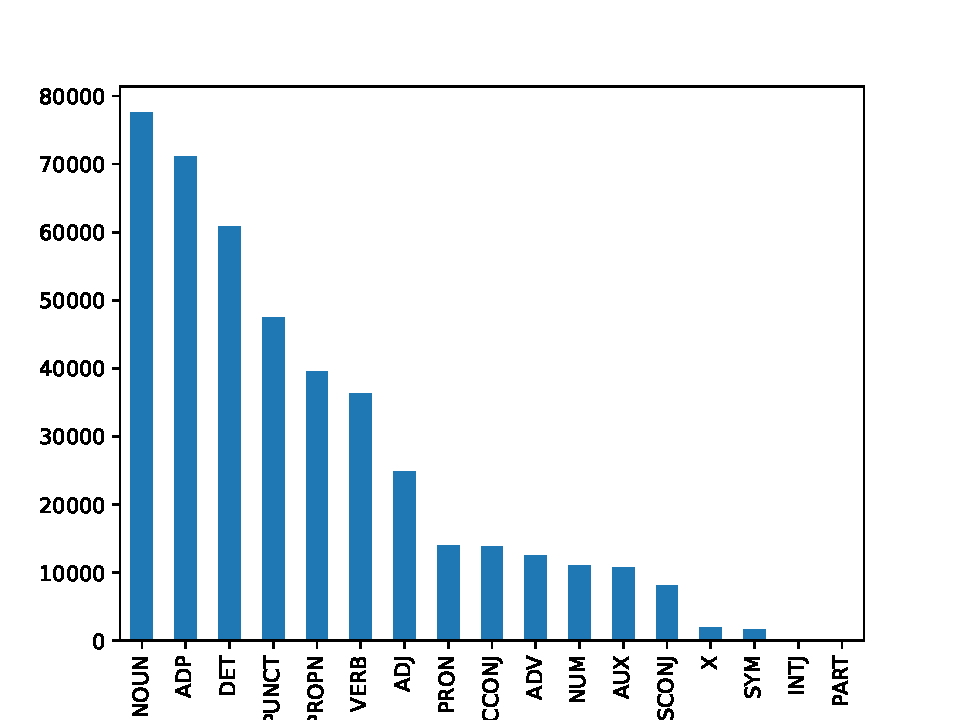
\includegraphics[width=\linewidth]{chart_es_upos.pdf}
  \end{center}
  \caption{Графік частот універсальних частин мови}
  \label{img:es_upos}
\end{figure}

\begin{figure}[H]
  \begin{center}
    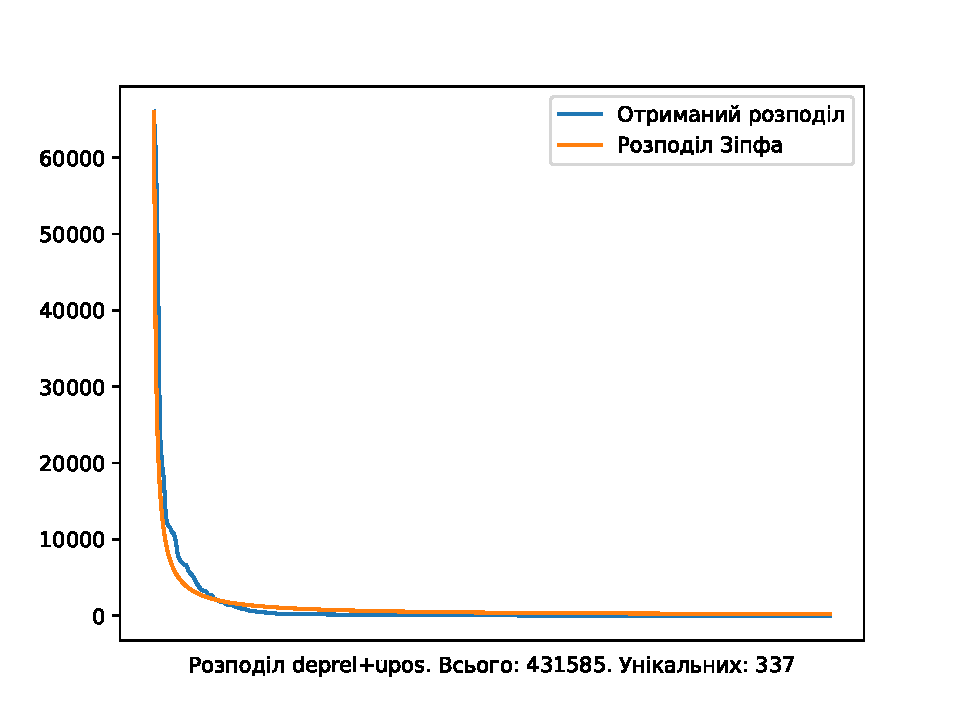
\includegraphics[width=\linewidth]{chart_es_deprel_upos.pdf}
  \end{center}
  \caption{Розподіл частин мови та універсального відношенння}
  \label{img:es_deprel_upos}
\end{figure}

\begin{figure}[H]
  \begin{center}
    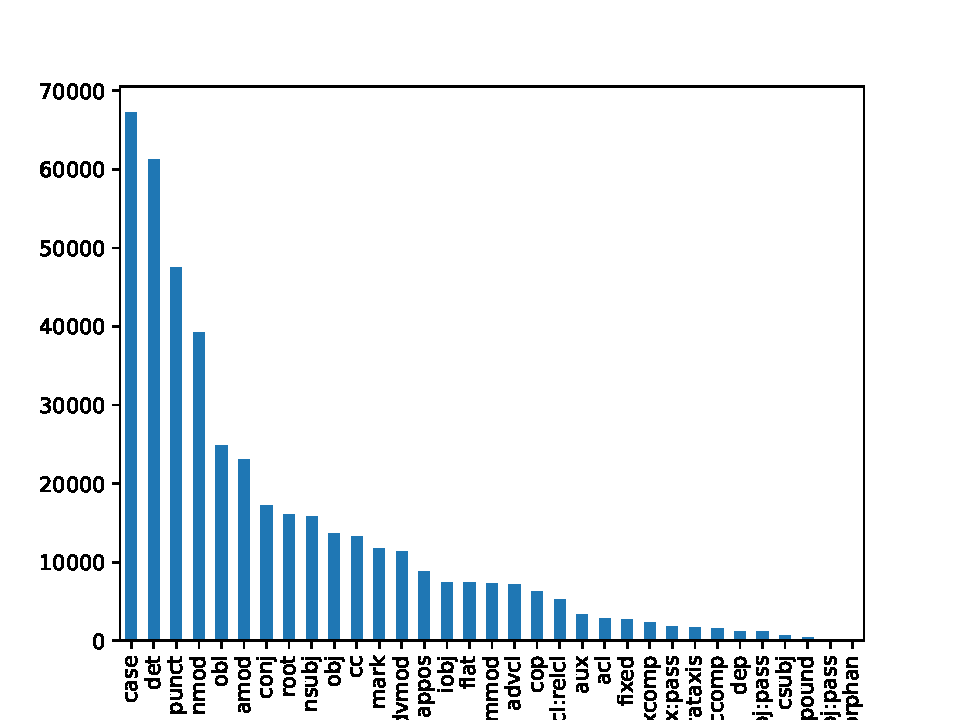
\includegraphics[width=\linewidth]{chart_es_deprel.pdf}
  \end{center}
  \caption{Розподіл універсальних відношенннь}
  \label{img:es0}
\end{figure}

\begin{figure}[H]
  \begin{center}
    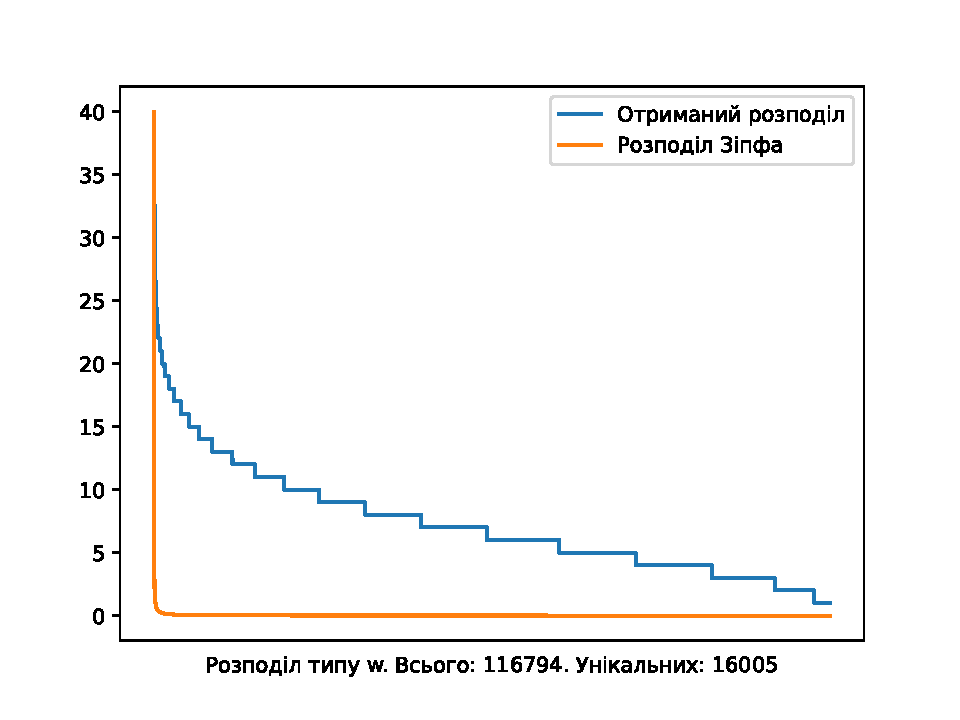
\includegraphics[width=\linewidth]{chart_es_type_w.pdf}
  \end{center}
  \caption{Розподіл піддерев токенів, що ростуть вшир}
  \label{img:es3}
\end{figure}

\end{multicols}

\newpage
\subsection{Розбір суфіксних дерев}
Для знаходження спільних характеристик дуже важливо мати
швидкий алгоритм пошуку по всім реченням корпусу. З цією метою,
всі речення трансформуються та подаються у вигляді суфікснних дерев, за 
алгоритмом Укконена. Таким чином операції з пошуку будуть здійснюватися за лінійнинй час.

\begin{figure}[ht]
  \begin{center}
    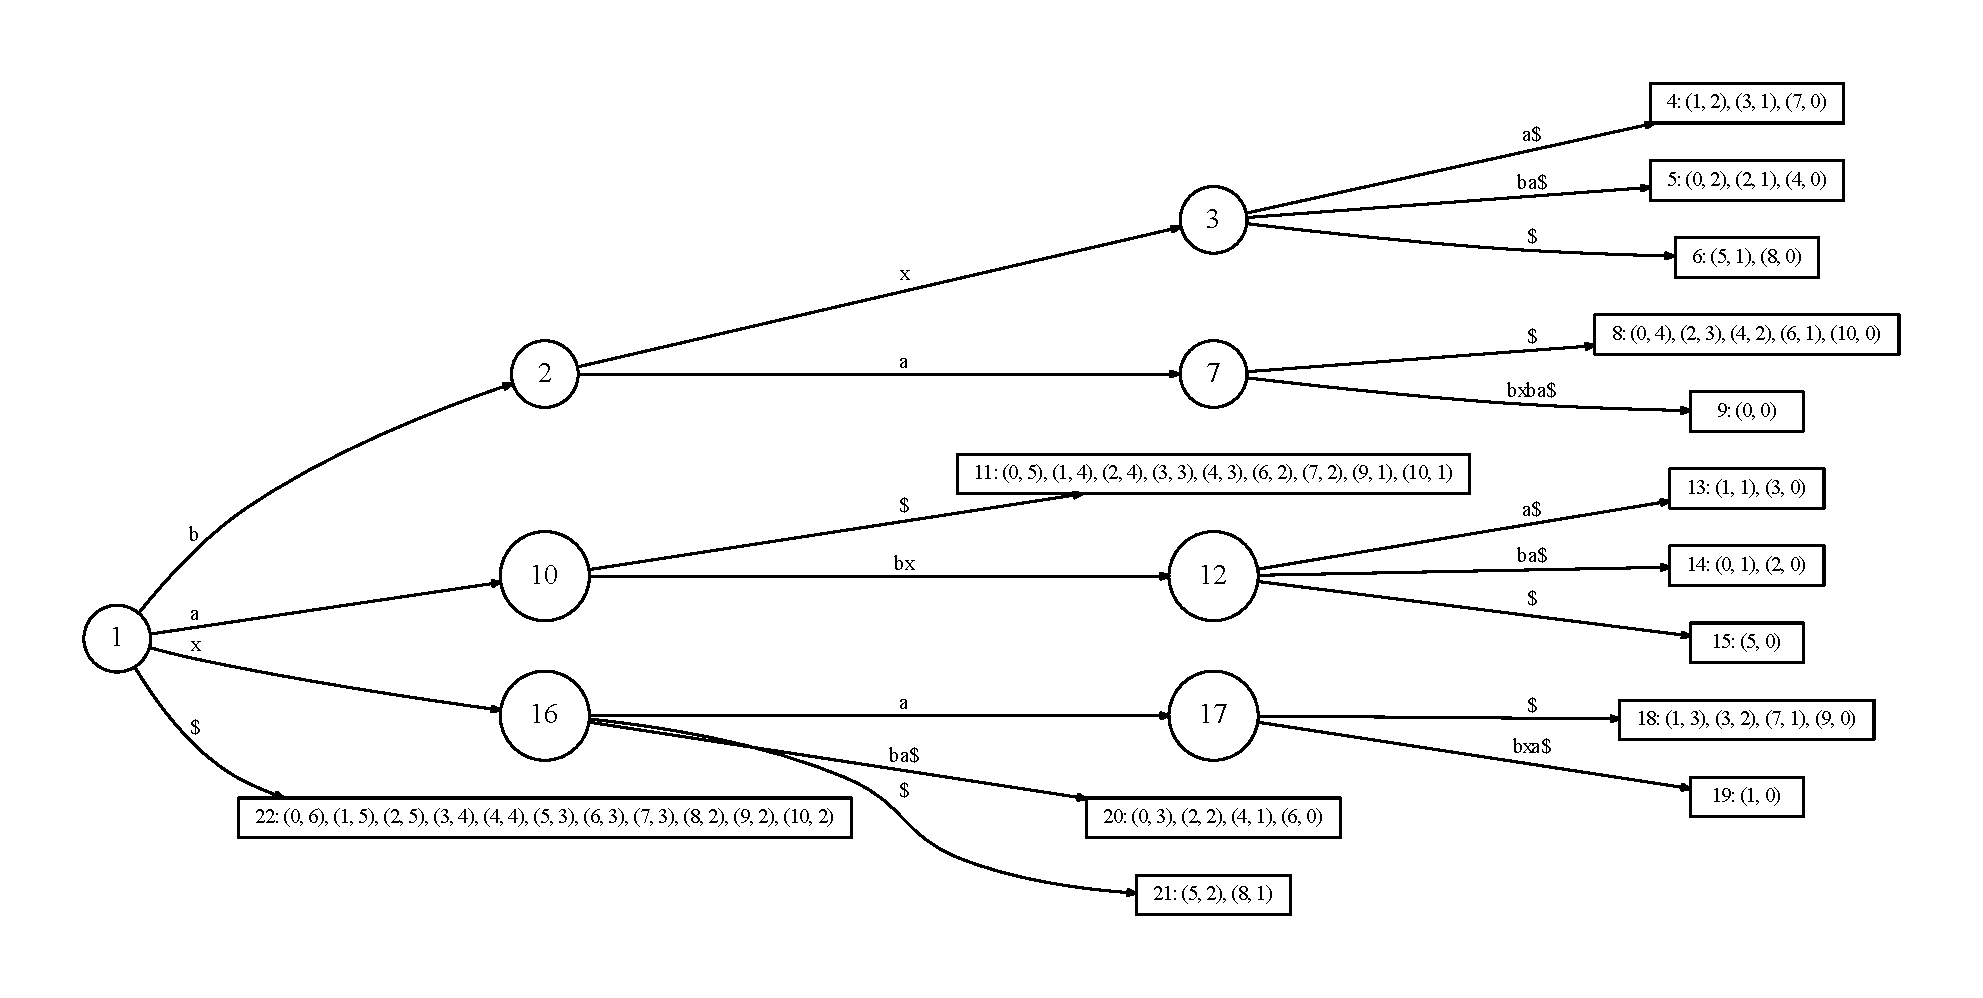
\includegraphics[width=\linewidth]{suffix_tree.pdf}
  \end{center}
  \caption{Суфікснне дерево}
  \label{img:suffix_tree}
\end{figure}

На рисунку \ref{img:suffix_tree} зображено приклад такого суфіксного дерева,
де видно, що суфікси є підрядками речень та подаються у вигляді індексів
вершин цього дерева.

Завдяки тому, що всі речення постають у вигляді суфіксного дерева, дуже просто
та швидко можна знаходити найбільш повторювані рядки, найдовші спільні
підрядки, найдовші паліндроми. Що значно розширює способи застосування
кінцевої програми.

Застосувавши описаний підхід до корпусу, перед цим подавши усі слова кожного
речення у вигляді універсальної частини мови, ми можемо знайти найдовші такі
підрядки та частоту їх зустрічання. Наприклад, для граматики
\texttt{NOUN~NOUN~NOUN~PROPN~ADP~ADJ~NOUN~ADJ~NOUN~NOUN~NUM~PUNCT} ми можемо
знайти відповідну грань у створеному суфіксному дереві - \texttt{BBBKHLBLBBND}.
Співставивши це із підрядками речень отримаємо результат: частота підрядків
із такою граматикою дорівнює трьом, а самі підрядки будуть виглядати наступним
чином: 
\begin{enumerate}
    \item \texttt{Міністерства охорони здоров’я України від 28 вересня 2012 року
    №~751~"}
    \item \texttt{постанови Кабінету Міністрів України від 25 березня 2009 року
    №~333~"}
    \item \texttt{постановою Кабінету Міністрів України від 25 березня 2009 року 
    №~333~"}
\end{enumerate}

Таким чином можна шукати спільні підрядки кожного речення корпусу, які
задовольняють певній граматиці. 


\subsection*{Висновки до розділу \arabic{section}}
\addcontentsline{toc}{subsection}{Висновки до розділу \arabic{section}}
Проаналізувавши отримані графіки, що зображено на рисунках
\ref{img:uk0}~\nobreakdash--~\ref{img:es3},
ми можемо дійти до висновку, що тренди, які
спостерігаються в україномовному корпусі майже так само прослідковуються в
іспаномовному корпусі, що підтверджує зазначену мету проекту Universal Dependencies.

У цьому розділі було продемонстровано статистичні закономірності у двох
корпусах UD. Загалом проаналізовано 2016 дерев в україномовному та 16013 дерев
в іспаномовному корпусах. Що в одному, що в іншому виявлено 17 унікальних
універсальних частин мови. А також було розібрано суфіксні дерева та проведено
пошук підрядів за заданою граматикою.